\begin{figure}[ht!]
    \begin{subfigure}{.5\textwidth}
    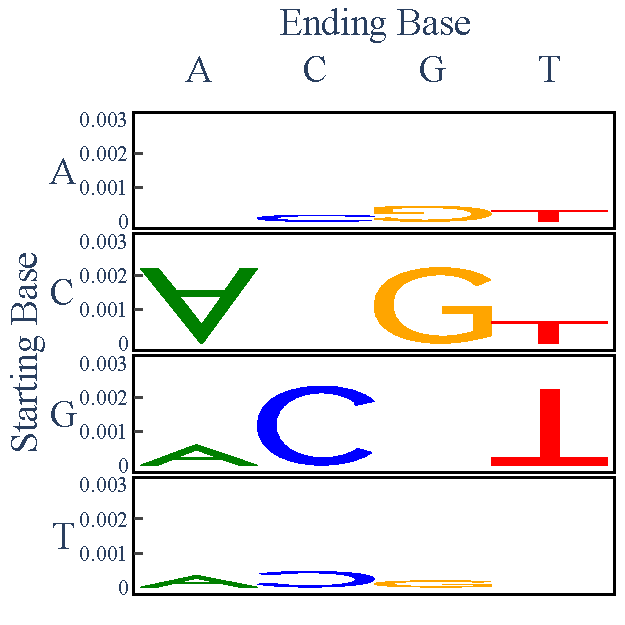
\includegraphics[scale=0.7]{graphics/spectra_CNS-Medullo_Lymph-BNHL.pdf}
    \caption{CNS-Medullo \textit{v.s.} Lymph-BNHL}
    \label{fig:spectra_medullo_bnhl}
    \end{subfigure}
    ~
    \begin{subfigure}{.5\textwidth}
    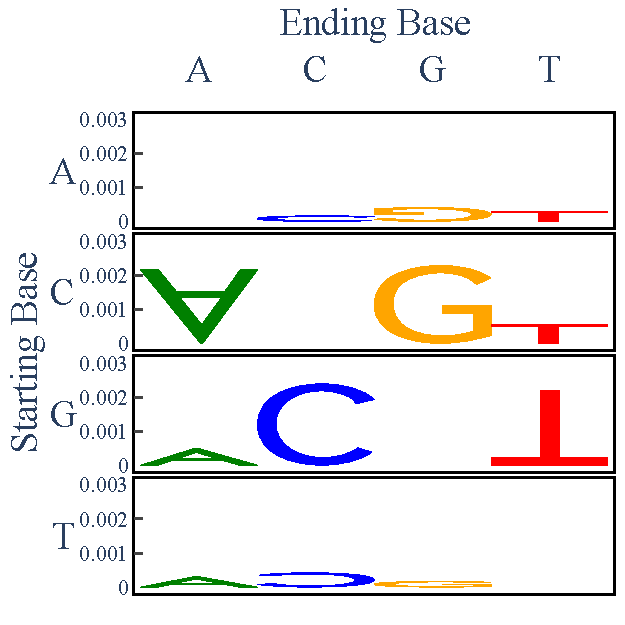
\includegraphics[scale=0.7]{graphics/spectra_CNS-Medullo_Lymph-CLL.pdf}
    \caption{CNS-Medullo \textit{v.s.} Lymph-CLL}
    \label{fig:spectra_medullo_cll}
    \end{subfigure} \\
    \vspace{0.5cm}
    
    \begin{subfigure}{.5\textwidth}
    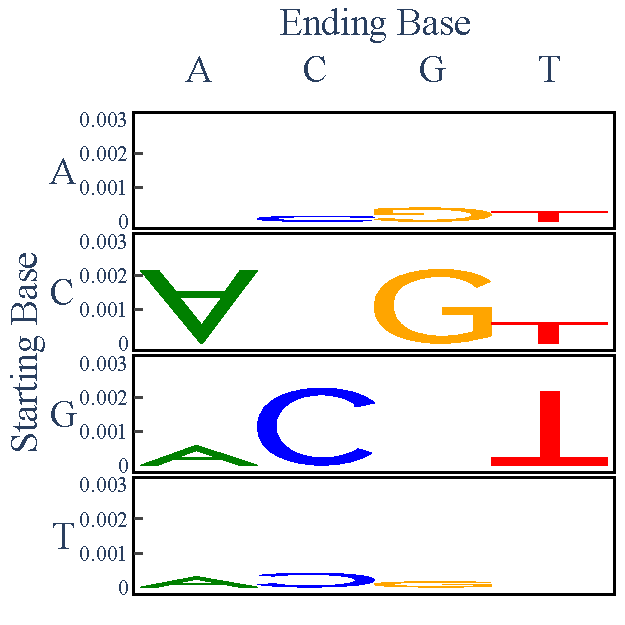
\includegraphics[scale=0.7]{graphics/spectra_CNS-PiloAstro_Lymph-CLL.pdf}
    \caption{CNS-PiloAstro \textit{v.s.} Lymph-CLL}
    \label{fig:spectra_piloastro_cll}
    \end{subfigure}
    ~
    \begin{subfigure}{.5\textwidth}
    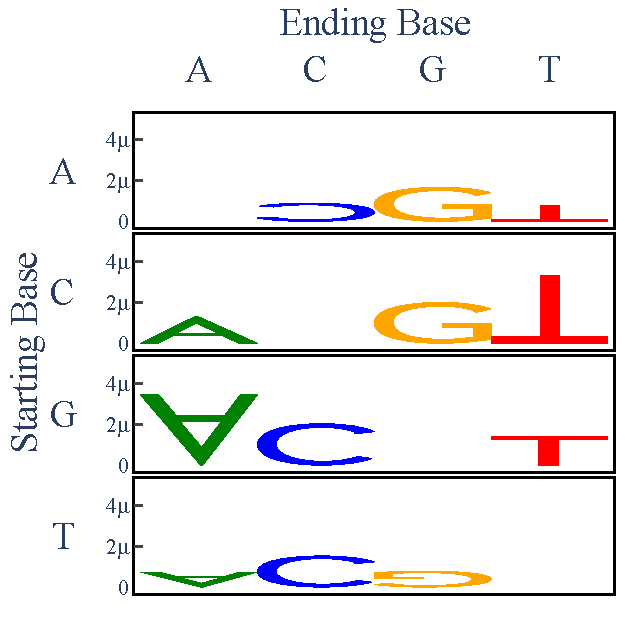
\includegraphics[scale=0.7]{graphics/spectra_Lymph-BNHL_Lymph-CLL.pdf}
    \caption{Lymph-BNHL \textit{v.s.} Lymph-CLL}
    \label{fig:spectra_bnhl_cll}
    \end{subfigure} \\
    \vspace{0.5cm}
    \caption{\textbf{Base substitutions are promising in discriminating cancers according to $RE$ between cancer pairs.} For each panel, each row was derived from a pair of GLMs. The x-axis is the wildtype base; the y-axis is the product of the substitution. The heights of the letters are $RE$'s. An up-orientation indicates an excess while a down-orientation indicates a deficit of the mutation when comparing the (a) CNS-Medullo to Lymph-BNHL, (b) CNS-Medullo to Lymph-CLL, (c) CNS-PiloAstro to Lymph-CLL, (d) Lymph-BNHL to Lymph-CLL. This is an extension of Figure \ref{fig:paired_spectra} in the main text.}
    \label{fig:apdx_paired_spectra}
\end{figure}